\documentclass[12pt]{article}

\usepackage{amsmath,amsthm,amssymb, stmaryrd, xcolor,graphicx,tikz}
\usepackage{comment}
\usepackage{cite}
\usepackage[pdftex]{hyperref}
\usetikzlibrary{graphs, positioning}

\begin{document}


\title{
    Order and Lattice Theorie
}

\author{
    Helmut Brandl
    \\
    \scriptsize (firstname dot lastname at gmx dot net)
}
\date{}

\maketitle


\abstract{
    Introduction to order and lattice theory.
}


\tableofcontents






\def\set#1{\left\{#1\right\}}
\def\powerset{{\mathcal P}}

\def\join{\sqcup}
\def\meet{\sqcap}
\def\bigjoin{\bigsqcup}
\def\bigmeet{\bigsqcap}
\def\downclosed{{\downarrow}}

\def\Nat{\mathbb N}

\def\lcm{\text{lcm}}
\def\gcd{\text{gcd}}


% Logic
\def\vertlist#1{
    \begin{array}{lllll}
    #1
    \end{array}
}

\def\bracklist#1{
    \left[ \vertlist{#1} \right]
}

\def\ruleh#1#2{\begin{array}{c} #1 \\ \hline #2\end{array}}
\def\rulev#1#2{\begin{array}{l} #1 \\ \hline #2\end{array}}

% Theorems
\theoremstyle{definition}
\newtheorem{definition}{Definition}[section] % envname, text, number base
\newtheorem{theorem}[definition]{Theorem}    % envname, parent counter, text
\newtheorem{lemma}[definition]{Lemma}
\newtheorem{corollary}[definition]{Corollary}
\newtheorem{example}[definition]{Example}
\newtheorem{remark}[definition]{Remark}



\section{Order}
%======================================================================


\begin{comment}
    - Order relation: reflexive, antisymmetric, transitive
    - Strict order
    - upper bound, upper bounds
    - greatest element: upper bound + in the set, def + uniqueness
    - least upper bound, def + uniqueness
    - maximal element
    - monotonic functions
    - cover relation -> hasse diagram
    - dual order

    - examples:

        - Mn
        - n-crown
        - partial maps
        - natural numbers
        - rational numbers (no hasse diagram

    - closure
        - operator: def idem, monotone, extensive, example ceiling
        - closure system: subset such that for all elements there is a least
        closed element above it
        - relation of both notions
        - galois connection
\end{comment}






\subsection{Basic Definitions}
%----------------------------------------------------------------------


\begin{definition}
    \label{defPoset}
    %------------------
    The pair $(S, \le)$ of a set $S$ and a relation $\le$ is called a
    \emph{partial order}
    %-------------------
    if the relation is
    \begin{enumerate}
        \item reflexive: $x \le x$

        \item antisymmetric: $x \le y \land y \le x \implies x = y$

        \item transitive $x \le y \land y \le z \implies x \le z$
    \end{enumerate}
    for all $x, y, z \in S$.
\end{definition}







\subsection{Special Elements}
%----------------------------------------------------------------------

\begin{definition}
    \label{defMinimalMaximalElement}
    %--------------------------------------------------

    An element $m \in A \subseteq P$ is a \emph{minimal element} in a subset $A$
    of a partial order $P$ if there is no strictly smaller element in the set
    $A$ i.e. $x \le a \implies x = a$ for all $x \in A$.


    An element $m \in A \subseteq P$ is a \emph{maximal element} in a subset $A$
    of a partial order $P$ if there is no strictly greate element in the set
    $A$ i.e. $a \le x \implies x = a$ for all $x \in A$.

\end{definition}



\begin{definition}
    \label{defUpperLowerBound}
    %------------------------------------------------------------

    Let $P$ be a partially ordered set and $A \subseteq P$ an arbitrary subset
    of $P$.

    An element $u \in P$ is called an \emph{upper bound} of $A$ if all elements
    in $A$ are less equal $u$ i.e. $\forall a\in A: a \le u$.

    An element $l \in P$ is called an \emph{lower bound} of $A$ if all elements
    in $A$ are greater equal $l$ i.e. $\forall a\in A: l \le a$.

    The set $A^u$ is the set of all upper bounds of $A$ and $A^l$ is the set of
    all lower bounds of $A$ i.e.
    $$
    \vertlist{
        A^u &:=& \set{x \in P: \forall a \in A: a \le x}
        \\
        A^l &:=& \set{x \in P: \forall a \in A: x \le a}
    }
    $$
\end{definition}



\begin{definition}
    \label{defMaximumMinimum}
    %--------------------------------------------------

    An element $m \in A$ of a subset $A \subseteq P$ of a partial order $(P,
    \le)$ is called a \emph{maximum} of $A$ if it is an upper bound of $A$ i.e.
    $m \in A^u$ and it is in the set $m \in A$.

    $m$ is called a \emph{minimum} of the set $A$ if it satisfies $m \in A^l$
    and $m \in A$.
\end{definition}

A maximum is in the intersection $A \cap A^u$, a minimum is in the intersection
$A \cap A^l$. Both intersections might be empty i.e. a maximum or a minimum of a
set $A$ might not exist.

If a maximum or a minimum of a set exists, then it is unique.

\begin{theorem}
    \label{thmMaximumMinimumUnique}
    \emph{Let $A \subseteq P$ of the partial order $(P, \le)$. A maximum or a
    minimum of the set $A$ (if it exists) is unique.
    }

    \begin{proof}
        Let $m, n \in P$ be two maxima of the set $A$. We have to show that both
        are equal. Since both are maxima we have $m, n \in A$ and $m,n \in A^u$.
        By definition~\ref{defUpperLowerBound} of $A^u$ we have $a \le m$ and $a
        \le n$ for all $a \in A$. This implies $m \le n$ and $n \le m$. An order
        relation is antisymmetric~\ref{defPoset} i.e. $m = n$ is valid.

        In the same manner the uniqueness of a minimum can be shown.
    \end{proof}
\end{theorem}


\begin{definition}
    \label{defSupremumInfimum}
    %--------------------------------------------------
    Let $A \subseteq P$ of the partial order $(P, \le)$.

    An element $m \in P$ is a \emph{supremum} or \emph{join} or \emph{least
    upper bound} of the set $A$ if $m$ is the minimum of $A^u$.

    An element $m \in P$ is an \emph{infimum} or \emph{meet} or \emph{greatest
    lower bound} of the set $A$ if $m$ is the maximum of $A^l$.

    Note that neither a minimum of $A^u$ nor a maximum of $A^l$ might exist.
    Therefore a join or a meet of a set $A$ might not exist.

    However of a join or a meet exists then it is unique because the maximum and
    minimum are unique~\ref{thmMaximumMinimumUnique}.

    If a join of a set $A$ exists it is written as $\bigjoin A$. If a meet of
    $A$ exists it is written as $\bigmeet A$. If the join or meet of the two
    element set $\set{a,b}$ exists we write $a \join b$ as the join of
    $\set{a,b}$ and $a \meet b$ as the meet of $\set{a,b}$
    %
    \footnote{In many texts the join of two elements is written as $a \lor b$
    and the meet as $a \land b$. Here this notation is not used to avoid
    confusion with the corresponding logical operators.}.
\end{definition}


\paragraph{Examples} Let's discuss the above definitions by looking at the
partial order

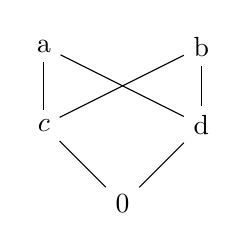
\begin{tikzpicture}
    \graph [branch right=2cm, grow up] {
        0 [xshift=1cm]
        -- {
            c/$c$ -- a,
            d -- b,
            c -- b,
            d -- a
        }
        %-- 1 [xshift=1cm];
    };
\end{tikzpicture}

\begin{enumerate}
    \item The upper bounds and the lower bounds of the empty set is the set of
        all elements of the partial order i.e.  $\emptyset^u = \emptyset^l =
        \set{0,a,b,c,d}$.

    \item For all singleton sets $\set{x}$ the element is contained in the
        upperbounds $x \in \set{x}^u$ and in the lower bounds $x \in \set{x}^l$
        of the singleton set. Therefore alll singleton sets have a maximum and a
        minimum. By definition the element is a singleton set is a minimal and a
        maximal element of the singleton set.

    \item The set $\set{a,b}$ does not have upper bounds i.e. $\set{a,b}^u =
        \emptyset$. But lower bounds exist $\set{a,b}^l = \set{c,d,0}$. Since
        $\set{a,b}^u$ is empty, the set $\set{a,b}$ does not have a join. The
        set of lower bounds is not empty, however $\set{c,d,0}$ does not have a
        maximum. Therefore $\set{a,b}$ does not have a meet either.

    \item
        Both $a$ and $b$ are maximal elements of the set of all elements.

    \item The set $\set{c,d}$ does have lower bound. It is a singleton set
        $\set{c,d} = \set{0}$. Since the element of a singleton set is the
        maximum and the minimum of the singleton set we conclude that the meet
        of $\set{c,d}$ exists i.e. we have $\bigmeet \set{c,d} = c \meet d = 0$.

    \item The element $0$ is a minimal element of the set of all elements. It is
        a minimum of the set of all elements as well.
\end{enumerate}






\subsection{Limit Element}
%----------------------------------------------------------------------

In infinite posets it is possible that an element $c$ has infinitely many
elements below it.

\begin{tikzpicture}
    \graph [grow up, branch right=2cm] {
        a0/$a_0$ -- a1/$a_1$ -- a2/$a_2$ --[dotted] c/$c$[xshift=1cm],
        b0/$b_0$ -- b1/$b_1$ -- b2/$b_2$ --[dotted] c
    };
\end{tikzpicture}

I.e. going upwards with a finite number of steps it is not possible to reach a
limit element. There are infinitely many steps needed to reach a limit element
from below. I.e. if you have an element $a_i < c$ then there exists always
another bigger element $a_{i+1}$ such that $a_i < a_{i+1} < c$.


If we take the natural numbers $\Nat$ and add a top element to it i.e. we use the
set $\set{0,1,2, \ldots, \infty}$ and use the usual order, then $\infty$ is a
limit element.

\begin{definition}
    \label{defLimitElement}
    %--------------------------------------------------

    An element $a$ is a limit element in a partial order if
    \begin{enumerate}
        \item it is not a minimal element of the order.

        \item for all $x < a$ there exists an $y$ with $x < y < a$
            i.e. $a$ has no immediate predecessor.
    \end{enumerate}

\end{definition}


\begin{theorem}
    \label{thmLimitElementIsJoin}
    \emph{A limit element $a$ in a partial order is the join of all elements
    strictly below it $a = \bigjoin \set{x: x < a}$.}

    \begin{proof}
        Let $A := \set{x: x < a}$.
        $a$ is certainly an upper bound for all elements strictly below it i.e
        $a \in A^u$. We have to prove that $a$ is the least element in $A^u$
        i.e. for all $b \in A^u$ we have  $a \le b$.

        Suppose there is a $b \in A^u$ with $b < a$. Then by definition of a
        limit element there exists an $x \in A$ with $b < x < a$. This
        contradicts the assumption that $b$ is an upper bound for all elements
        in $A$. Therefore such a $b$ cannot exist.
    \end{proof}
\end{theorem}

\section{Lattices}
%======================================================================


\begin{comment}
    - semilattice
        - def: order with infimum (meet)
        - def: algebraic: idempotent, commutative, associative (commutative
        semigroup)
        - both defs are equivalent
        - finite meet semilattices have least element: meet of all elements
    - lattice
        - two definitions and equivalence
        - lattice from a finite meet semilattice with greatest element
    - complete lattices
        - meet semilattice
        - complete meet semilattice is a complete lattice
        - Knaster-Tarski
\end{comment}

% Non lattice
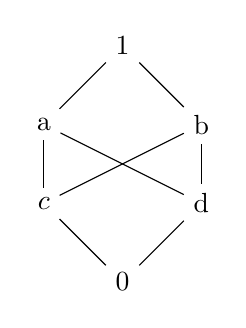
\begin{tikzpicture}
    \graph [branch right=2cm, grow up] {
        0 [xshift=1cm]
        -- {
            c/$c$ -- a,
            d -- b,
            c -- b,
            d -- a
        }
        -- 1 [xshift=1cm];
    };
\end{tikzpicture}

The lower bounds of $\set{a,b}$ are $\set{0,c,d}$, but there is no greatest
lower bound $a \land b$. The upper bounds of $\set{c,d}$ are $\set{a,b,1}$, but
there is no least upper bound $c \lor d$.



\begin{theorem}
    \label{thmOneDistributivitySufficient}
    \emph{In a lattice the distributivity of join over meet implies the
    distributivity of meet over join (note: join and meet are dual operations,
    therefore the other direction can be proved in the same manner).
    }

    \begin{proof}
        Assume $x \join (y \meet z) = (x \join y) \meet (x \join z)$. We have to
        prove $x \meet (y \join z) = (x \meet y) \join (x \meet z)$.

        $$
        \vertlist{
            x \meet (y \join z)
            &=&
            (x \meet (x \join z)) \meet (y \join z)
            & \text{absorption}
            \\
            &=&
            x \meet ((x \join z) \meet (y \join z))
            & \text{associativity}
            \\
            &=&
            x \meet ((z \join x) \meet (z \join y))
            & \text{commutativity}
            \\
            &=&
            x \meet (z \join (x \meet y))
            & \text{assumption}
            \\
            &=&
            x \meet ((x \meet y) \join z)
            & \text{commutativity}
            \\
            &=&
            ((x \meet y) \join x) \meet ((x \meet y) \join z)
            & \text{absorption}
            \\
            &=&
            (x \meet y) \join (x \meet z)
            &\text{assumption}
        }
        $$
    \end{proof}
\end{theorem}



\subsection{Distributive Lattices}
%======================================================================



\subsubsection{Some Examples}
%----------------------------------------------------------------------

\begin{enumerate}
    \item The set of natural numbers $\set{0, 1, 2, 3, \ldots}$ with the usual order
        is a distributive lattice.
        The join of two elements is the maximum of two elements, the meet is its
        minimum. The lattice is not complete, because the set of all numbers has
        no join and the meet of the empty set does not exist (the meet of the
        empty set is greatest element and the natural numbers have no greatest
        element).

        The lattice does not have infinite descending chains, so it is a DCC
        lattice. However it has infinitely ascending chains.


    \item The set of natural numbers with an added top element
        $$\set{0, 1, 2, 3, \ldots, \infty}$$
        is a complete distributive DCC lattice.

        The lattice is complete because all subsets have a meet and a join. The
        meet of the
        empty set is the top element $\bigjoin \emptyset = \infty$, the join of
        a finite set is its greatest element, the join of an infinite set is the
        top element.

    \item Consider he cofinite subset lattice of the natural numbers which is
        the set of all finite subsets of the natural numbers with the top
        element which is the set of all numbers. The join and meet operation are
        union and intersection.

        This lattice is complete and distributive. It is complete because of the
        top element, it is distributive because set union and intersection are
        distributive.

        The atoms of this lattice are the singleton sets $\set{0}$, $\set{1}$,
        $\ldots$. There are infinitely many atoms therefore the width of the
        lattice is infinite.

        The lattice satisfies the descending chain condition. If you start a
        descending chain with a finite set of natural numbers there are
        evidently only finite steps downwards to reach the empty set. If you
        start a descending chain at the top, the next downward element is a
        finite set (there are no infinite sets strictly below the top element).
        From the second element in the downward chain there are only finitely
        many downward steps possible before reaching the bottom element (the
        empty set).


    \item The powerset of the set of natural numbers is a complete distributive
        lattice as well. As in the previuos example the top element is the set
        of all natural numbers.

        However this lattice has proper infinite subsets. E.g. the set of all
        even numbers, the set of all prime numbers, the set of all powers of a
        certain prime number.

        Interestingly this lattice does not satisfy the descending chain
        condition. It is easy to construct an infinitely descending chain.
        $$
        \vertlist{
            \set{0, 1, 2, 3, \ldots}
            \\
            \supset \set{1, 2, 3, \ldots}
            \\
            \supset \set{2, 3, \ldots}
            \\
            \ldots
        }
        $$
        The trick is to start with an infinite set and remove at each downward
        step one element of the set. Since removing one element of an infinite
        set does not change its infiniteness and the descending chain never ends.

    \item The divisibility lattice of the natural numbers is a complete
        distributive DCC lattice.

        The elements of the lattice are the natural number ordered by
        divisibility. We say that $a$ divides $b$ if there is a number $n$ such
        that $a n = b$ is valid. Not that $1$ is the least element, because $1$
        divides all numbers ($1 b = b$) and $0$ is the top element because all
        numbers divide 0 ($a 0 = 0$).
\end{enumerate}


\begin{theorem}
    \label{thmChainsAreDistributive}
    %--------------------------------------------------
    \emph{All chain lattices are distributive.}

    \begin{proof}
        The join of two elements is their maximum, the meet of two elements is
        their minimum. We have to prove
        $$
            max(a, min(b, c)) = min(max(a,b), max(a,c))
        $$
        We consider 3 cases:
        \begin{enumerate}
            \item $a$ is the smallest:
                $$
                \vertlist{
                    max(a, min(b,c)) &=& min(b,c)
                    \\
                    min(max(a,b), max(a,c)) &=& min(b,c)
                }
                $$

            \item $a$ is the greatest:
                $$
                \vertlist{
                    max(a, min(b,c)) &=& a
                    \\
                    min(max(a,b), max(a,c)) &=& a
                }
                $$

            \item $a$ is between $b$ and $c$:
                \begin{enumerate}
                    \item $b \le a \le c$:
                    $$
                    \vertlist{
                        max(a, min(b,c)) &=& a
                        \\
                        min(max(a,b), max(a,c)) &=& a
                    }
                    $$

                    \item $c \le a \le b$:
                    $$
                    \vertlist{
                        max(a, min(b,c)) &=& a
                        \\
                        min(max(a,b), max(a,c)) &=& a 
                    }
                    $$
                \end{enumerate}

        \end{enumerate}
    \end{proof}
\end{theorem}




\subsection{Join Irreducible Elements}
%======================================================================


In some lattices it is possible to find some basic elements such that all other
elements can be generated by forming joins over the basic elements. I.e. we search
for a set of elements $B$ such that every element $e$ of the lattice can be
generated by $e = b_0 \join b_1 \join \ldots \join b_{n-1}$ where all $b_i \in
B$. The basic elements $B$ are similar to the prime numbers in number theory
where each natural number can be represented by a product of prime numbers.

Prime numbers are numbers which cannot be represented as product of different
other numbers. If a prime number $p$ is a product of the form $p = ab$, then it
is either $a$ or $b$.

In a similar manner we define join irreducible elements as elements which cannot be
represented as a join of other elements of the lattice.


\begin{definition}
    % Join Irreducible
    % ----------------
    \label{defJoinIrreducible}
    We give two definitions of \emph{join irreducible} elements and show that
    both definitions are equivalent.

    \begin{enumerate}
        \item An element $q$ of a lattice $L$ is \emph{join irreducible} if it is
            not the least element of the lattice and for all elements $a,b \in L$ we
            have $\ruleh{q = a \join b}{q = a \lor q = b}$. I.e. if $q$ is the
            join of two elements, then it is one of the elements.
    
        \item An element $q$ of a lattice $L$ is \emph{join irreducible} if for
            all finite sets $F \subseteq L$ we have $q = \bigjoin F \implies q \in
            F$. I.e. if $q$ is the join of finitely many elements of the
            lattice then it is one of these elements.
    \end{enumerate}


    \begin{proof} We prove the equivalence of both definitions. 
        \begin{enumerate}
            \item First we show that a join irreducible element $q$ in the first
                definition is also join irreducible in the second definition.

                Assume that $q$ is join irreducible according to the first
                definition and $q = \bigjoin F$ for some finite set $F$. We prove
                that $q \in F$ by induction on the size $n$ of the set.

                In the base case $F$ is the empty set. This implies that $q$ is
                the least element of the lattice which contradicts the fact the
                $q$ is join irreducible according to the first definition. Ex
                falso quodlibet i.e. the claim is proved in the base case.

                Assume that $q = \bigjoin F \implies q \in F$ for $|F| = n$ and
                that $q = \bigjoin (\set{a} \cup F) = a \join (\bigjoin F)$. Since
                $q$ is join irreducible according to the first definition we
                have $q = a \lor q = \bigjoin F$. If $q = a$ then $q \in (\set{a}
                \cup F)$. If $q = \bigjoin F$ then by the induction hypothesis $q
                \in F$ and therefore $q \in (\set q \cup F)$.


            \item Now we assume that $q$ is join irreducible according to the
                second definition. Assume $q = a \join b$. We take $F :=
                \set{a,b}$. Then $q \in F$ according to the second definition. So
                $q$ is join irreducible according the first definition.
        \end{enumerate}

    \end{proof}
\end{definition}




\paragraph{Examples}
%------------------------------------------------------------
\begin{enumerate}
    \item In a chain e.g. with numbers $\set{1,2,3,4}$ with the standard order
        all numbers except the smallest number are join irreducible.
        In such a linear order the join of two elements is the maximum of the
        elements. I.e. an element can be the join of two elements only if it is
        greater than the other. Therefore it is one of the elements.

        The concept of join irreducibility in a chain is relatively boring,
        because all elements are join irreducible and only the least one (if it
        exists) can be represented as a join $\bigjoin \emptyset$.

        Even if the chain contains limit elements, then the limit elements are join
        irreducible as well. In an infinite chain with no least elements all
        elements are join irreducible.

    \item In a powerset lattice $\powerset{\set{a,b,c}}$ (join is union) only
        the singleton sets $\set{a}$, $\set{b}$ and $\set{c}$ are join
        irreducible. All other sets can be generated by joining finitely many
        singleton sets.

        The singleton sets are join irreducible, because the only join which
        creates a singleton set is $\emptyset \cup \set a$ (or $\set{a} \cup
        \emptyset$) and the singleton set is clearly one of the joined sets.

        The other sets like $\set{a,b}$ are join reducible because we have
        $\set{a,b} = \set{a} \cup \set{b}$.

    \item Limit elements in chains are join irreducible. Consider a limit
        element $c$ such that $c = a \join b$. In a chain the join operation
        returns the maximum of both elements i.e. the join is the maximum of the
        set $\set{a,b}$ and therefore one of the two elements. This is the
        definition of a join irreducible element.

    \item A limit element in general is not join irreducible. Consider the
        lattice

        \begin{tikzpicture}
            \graph [grow up, branch right=2cm] {
                0/$0$[xshift=1cm]
                -- {
                    a0/$a_0$ -- a1/$a_1$,
                    b0/$b_0$ -- b1/$b_1$
                }
                --[dotted] 1/$1$[xshift=1cm];
            };
        \end{tikzpicture}

        Note that $1 = a_i \join b_j$ and $1$ is neither $a_i$ nor $b_j$ for any
        values of $i$ and $j$. So the limit element $1$ can be generated by a
        join of a finite set of elements.
\end{enumerate}





\paragraph{DCC lattices}
%----------------------------------------------------------------------
Join irreducible elements play an important role in lattices satisfying the
descending chain condition. All elements of such a lattice can be constructed by
using joins of a finite set of join irreducible elements.


\begin{theorem}
    \label{thmDCCJoinIrreducible}
    %-------------------------------------------------------------------------
    \emph{If a lattice $L$ satisfies the descending chain condition (DCC), then
    every element of $L$ is the join of finitely many join irreducible
    elements.}

    \begin{proof}
        \begin{enumerate}
            \item Suppose there is an element of $L$ which is not the join of
                finitely many join irreducible elements. Because of the
                descending chain condition there exists a minimal element $m$
                which is not the join of finitely many join irreducibles.

            \item $m$ is not join irreducible. Otherwise we would have $m =
                \bigjoin \set{m}$ and $m$ would be the join of a finite set of
                join irreducibles.

            \item Since $m$ is not join irreducible there exist two elements $a$
                and $b$ which are different from $m$ such that $m$ is the join
                of these two elements $m = a \join b$. These two elements are
                strictly below $m$.

            \item $m$ is minimal in the set of elements which are not the join
                of a finite set of join irreducibles. So $a$ and $b$, which are
                strictly below $m$, are the join of join irreducibles. Say $a =
                \bigjoin A$ and $b = \bigjoin B$ where $A$ and $B$ are finite
                sets of join irreducibles. This fact implies $m = a \join b =
                \bigjoin (A \cup B)$ and contradicts the assumption that $m$
                is not the join of a finite set of join irreducibles.

            \item Therefore an element which is not the join of a finite set of
                join irreducibles cannot exist.
        \end{enumerate}
    \end{proof}
\end{theorem}


The join irreducible elements of a lattice $L$ with DCC have another nice
property. All elements of the lattice are the join of all join irreducibles
below it.

\begin{theorem}
    \label{thmJoinOfJoinIrreduciblesBelow}
    \emph{ Let $L$ be a lattice satisfying the descending chain condition,
    $J(L)$ the set of all join irreducibles of $L$ and $\phi$ be the function
    which maps all elements to the set of join irreducibles below it $\phi(a) =
    \set{p \in J(L): p \le a}$. Then $a = \bigjoin(\phi(a))$.}

    \begin{proof}
        We prove the claim by contradiction assuming there is an element $a$
        which is not equal to $\phi(a)$. Since the lattice satisfies DCC there
        is a minimal element $m \ne \phi(m)$.

        We have to distinguish the cases that $m$ is join irreducible or not.

        \begin{enumerate}
            \item $m$ is join irreducible:

                In this case $m \in \phi(m)$ and therefore $m \le
                \bigjoin(\phi(m))$. By definition of $\phi$ $m$ is an upper
                bound for $\phi(m)$. Since a join is the least upper bound we
                have $\bigjoin(\phi(m)) \le m$. So $m = \bigjoin(\phi(m)$ which
                contradicts the assumption $m \ne \bigjoin(\phi(m))$


            \item $m$ is not join irreducible:

                In this case there exist $a,b \in L$ different from $m$ such
                that $m = a \join b$.  Because $m$ is minimal we have $a =
                \bigjoin(\phi(a))$ and $b = \bigjoin(\phi(b))$.

                This implies $m = \bigjoin(\phi(a) \cup \phi(b))$.

                We know that $a \le m$ and $b \le m$ ($m$ is the least upper
                bound) and therefore $\phi(a) \cup \phi(b) \subseteq \phi(m)$.
                Therefore $m \le \bigjoin(\phi(m))$.

                By definition $m$ is an upperbound for $\phi(m)$ i.e.
                $\bigjoin(\phi(m)) \le m$.

                This implies $m = \bigjoin(\phi(m))$ which contradicts the
                assumption that $m$ is not the join of all join irreducibles
                below it.
        \end{enumerate}
    \end{proof}
\end{theorem}







\subsection{Join Prime Elements}
%================================================================================




\paragraph{Prime property}
%----------------------------------------------------------------------
If a lattice is distributive
then the join irreducibles have the prime property which says whenever a join
irreducible element is below a join of a finite set of elements, then there
exist an element in the finite set which is an upper bound of the join
irreducible.

In nondistributive lattices this prime property is not guaranteed. Consider the
diamond lattice $M_3$ and the pentagon lattice $N_5$.

    \tikz
    \graph [grow up, branch right=1cm] {
        0/$0$[xshift=1cm]
        -- {
            a/$a$,
            b/$b$,
            c/$c$
        }
        -- 1/$1$[xshift=1cm];
    };
%
    \tikz
    \graph [grow up, branch right=2cm] {
        0/$0$[xshift=1cm]
        -- {
            a/$a$,
            b/$b$ -- c/$c$
        }
        -- 1/$1$[xshift=1cm];
    };

The elements $a$ $b$ and $c$ are join irreducible. In both cases we have $c \le
\bigjoin\set{a,b}$. The prime property would require either $c \le a$ or $c \le
b$. None of the statements is valid.

In the diamond lattice $M_3$ neither of the middle elements $a,b,c$ have the
prime property. In the pentagon lattice $N_5$ $a$ and $b$ have the prime
property, but $c$ does not.

In distributive lattices all join irreducibles have the prime property.

Let us first give a formal definition of join prime elements.

\begin{definition}
    \label{defJoinPrime}
    %------------------------------------------------------------
    We give 2 definitions of \emph{join prime} elements and show that both
    definitions are equivalent.

    \begin{enumerate}
        \item An element $p$ of a lattice $L$ is \emph{join prime} if for any
            finite set $F \subseteq L$ of elements where $p$ is below the join of
            these elements $p \le \bigjoin F$, then there exist an element $a
            \in F$ such that $p \le a$.

        \item An element $p$ of a lattice $L$ is \emph{join prime} if it is not
            the least element of the lattice and if for all $a,b \in L$ where
            $p$ is below the join of the elements $p \le a \join b$ then $p$ is
            below one of the elements i.e. $p \le a$ or $p \le b$ is satisfied.
    \end{enumerate}

    \begin{proof}
        First we prove that the first definition implies the second and then the
        other way round.

        \begin{enumerate}
            \item $1 \implies 2$: Assume that $p$ is join prime according to the
                first definition.

                \begin{itemize}
                    \item $p$ is not the least element of the lattice: Assume
                        that $p$ is the least element of the lattice. Then $p
                        \le \bigjoin \emptyset$ because $\bigjoin \emptyset$ is
                        the least element of the lattice. The first definition
                        requires that there is an element $a \in \emptyset$.
                        This is not possible, therefore $p$ cannot be the least
                        element of the lattice.

                    \item Assume $p \le a \join b$. This is equivalent to $p \le
                        \set{a,b}$. The first definition requires that either $p
                        \le a$ or $p \le b$ is valid.
                \end{itemize}

            \item $2 \implies 1$: Assume that $p$ is join prime according to the
                second definition. We have to proof that for all finite sets $F
                \subseteq L$ that $p \le \bigjoin F \implies \exists a \in F: p
                \le a$. We prove this by induction on the size of $F$.

                \begin{itemize}
                    \item Base case $F = \emptyset$. Assume $p \le \join
                        \emptyset$. This implies that $p$ is the least element
                        of the lattice. This contradicts the fact that $p$ is
                        join prime according to the first definition. Ex falso
                        quodlibet, therefore the claim is valid in the base
                        case.

                    \item Induction step: Assume that the claim is valid for $F$
                        and $p \le \bigjoin(\set{a} \cup F)$. This is equivalent
                        to $p \le a \join (\bigjoin F)$. The second definition
                        requires that $p \le a$ or $p \le \bigjoin F$.

                        In the first case we have already found an element $a$ in
                        $\set{a} \cup F$ such that $p \le a$.

                        In the second case the induction hypothesis guarantees
                        an element $a \in F$ such that $p \le a$.
                \end{itemize}
        \end{enumerate}
    \end{proof}
\end{definition}



The property of being join prime is stronger than the property of being join
irreducible.

\begin{theorem}
    \emph{In an arbitrary lattice $L$ all join prime elements are join
    irreducible.}

    \begin{proof}
        Assume that an element $p$ is join prime. We prove that $p$ is join
        irreducible~\ref{defJoinIrreducible}.

        \begin{enumerate}
            \item $p$ is not the least element of $L$: Trivial by definition.

            \item Assume $p = a \join b$. We have to show that $p$ is either $a$
                or $b$.

                Since $p$ is join prime and $p \le a \join b$ we have either $p
                \le a$ or $p \le b$.

                Assume $p \le a$. Since $p$ is the join of $a$ and $b$ we have
                $a \le b$ and infer by antisymmetrie $p = a$. This proves the
                claim.

                Assume $p \le b$. By the same reasoning we get $p = b$ and the
                claim is valid.
        \end{enumerate}
    \end{proof}
\end{theorem}


We have seen that all join prime elements are join irreducible as well. But not
all join irreducibles are join prime as we have seen for the diamond lattice
$M_3$ and the pentagon lattice $N_5$. But for distributive lattices we can prove
that all join irreducibles are join prime.


\begin{theorem}
    \label{thmDistributiveJoinIrreducibleIsJoinPrime}
    %----------------------------------------------------------------------
    \emph{In a distributive lattice $L$ all join irreducible elements $p$ are
    join prime. }

    \begin{proof}
        We have to show
        \begin{enumerate}
            \item $p$ is not the least elements of the lattice $L$: Trivial by
                definition~\ref{defJoinIrreducible}.

            \item If $p \le a \join b$ then $p \le a$ or $p \le b$:

                Assume $p \le a \join b$. By definition of the order relation in
                a lattice we have $p = p \meet (a \join b)$. Because of
                distributivity we have $p = (p \meet a) \join (p \meet b)$. $p$
                is join irreducible~\ref{defJoinIrreducible} so we have either
                $p = p \meet a$ or $p = p \meet b$ which by definition of the
                order relation implies $p \le a$ or $p \le b$.
        \end{enumerate}
    \end{proof}

    Note that the distributivity of the lattice is essential.
\end{theorem}


\paragraph{Unique join of join irreducibles}
%----------------------------------------------------------------------
In the special case of distributive lattices satisfying DCC each element can be
constructed in a unique manner as a join of join irreducibles.

In the divisibility lattice of the natural number $12$ the lattice elements are
$\set{1,2,4,3,6,12}$. The prime powers $\set{2,4,3}$ are join irreducible. The
join operation is the least common multiple $\lcm $ operation.

Let's consider the
join irreducibles generating the number $12$. At first glance we have two
possibilities $12 = \lcm(2,3,4) = \lcm(3,4)$. However the operation
$\lcm(2,3,4)$ is somewhat redundant since $2$ is a factor of $4$ and is
therefore not needed.

If we restrict ourselves to antichains of join irreducibles we can exclude
$\lcm(2,3,4)$ because it is not an antichain. By regarding only antichains of
join irreducibles the number $12$ has the unique factorisation $12 = \lcm(3,4)$.

\begin{theorem}
    \label{thmDistributiveDCCUniqueJoin}
    \emph{
        In a distributive lattice satisfying the descending chain condition
        every element can be represented as a unique join of of a finite
        antichain of join irreducibles.
    }

    \begin{proof} Assume that an element
        $a$ can be represented by two finite antichains $P$ and $Q$ of join
        irreducibles i.e. $a = \bigjoin P = \bigjoin Q$. We prove $P \subseteq
        Q$. The proof of $Q \subseteq P$ is similar and both prove that the
        representation is unique.

        Assume $p \in P$:
        \begin{enumerate}
            \item Since $p \le \bigjoin P$ we have $p \le \bigjoin Q$ as well.

            \item By the prime
                property~\ref{thmDistributiveJoinIrreducibleIsJoinPrime}
                there is some $q \in Q$ such that $p \le q$.

            \item By the same reasoning there exists a $p' \in P$ such that $q \le
                p'$.

            \item This gives us $p \le q \le p'$. $P$ being an antichain
                guarantees $p = p'$ and therefore $p = q$.

            \item So $p \in Q$ for all $p \in P$.
        \end{enumerate}
    \end{proof}
\end{theorem}


We have already seen that distributivity and the descending chain condition give
us a lot of nice properties of the join irreducibles. If we restrict ourselves
to complete lattices (note: all finite lattices are complete) then we get the
strong property that no infinite antichain of join irreducibles exists. I.e. the
lattice can grow upwards arbitrarily, but not downwards and not in width.

\begin{theorem}
    \label{thmNoInfiniteAntichainJoinIrreducible}
    %------------------------------------------------------------
    \emph{ Let $L$ be a complete distributive lattice satisfying the descending
    chain condition. The all antichains of join irreducibles are finite.}

    \begin{proof}
        Let's assume there is an infinite antichain $\set{p_0, p_1, p_2,
        \ldots} \subseteq L$ of join irreducibles. Using this antichain we
        construct an infinitely descending chain which contradicts the
        descending chain condition.

        Let $x_0, x_1, x_2, \ldots$ be defined as $x_i := \bigjoin \set{p_i, p_{i+1},
        \ldots} = \bigjoin \set{p_k: i \le k}$. This implies $x_i = p_i \join
        x_{i+1}$. $x_i$ is therefore an upperbound for $x_{i+1}$ and we have
        $x_i \ge x_{i+1}$. So the series is descending.

        Now we proof that the series is strictly descending i.e. $x_i >
        x_{i+1}$. Assume the opposite i.e. for some $i$ we have $x_i = x_{i+1}$.
        In this case the condition $x_i = p_i \join x_{i+1}$ gives $x_{i} = p_i
        \join x_i$. According to the order relation of a lattice this implies
        $p_i \le x_{i}$.

        WRONG / WRONG: Not strictly descending!!
    \end{proof}
\end{theorem}






\subsection{Compact Elements}
%======================================================================

\begin{comment}
    Missing Proofs:

    - In a distributive complete lattice with DCC all join irreducibles are
    compact: This is NOT VALID. Counterexample: Natural numbers with top. The
    top element is join irreducible but not compact!!!
\end{comment}

\paragraph{Examples}
\begin{enumerate}
    \item The least element $0$ in a lattice is compact, because $0 = \bigjoin
        \emptyset$ and the empty set is finite.

    \item All elements in a finite lattice are trivially compact.

    \item Consider the real interval $[0,1]$ with the usual order. It is
        complete lattice because every subset has a supremum.

        Only the number $0$ is compact. The only possibilities to represent $0$
        as a join are $0 = \bigjoin \emptyset$ and $0 = \bigjoin \set{0}$. As
        soon as there is an element different from $0$ in the set, the join is
        strictly above $0$.

        All the other numbers are not compact. Consider the set
        $$
        D := \set{0, \frac 1 2 a, \frac 2 3 a, \ldots, \frac i {i+1} a, \ldots}
        $$
        with $0 < a$. The elements in the set come arbitrarily close to $a$ but
        never reach it. $a$ is the supremum of the set and in particular $a \le
        \bigjoin D$. However there is no finite subset $F \subseteq D$ with $a
        \le \bigjoin F$.

    \item Consider the lattice

        \begin{tikzpicture}
            \graph [grow up, branch right=2cm] {
                a/$a$ [yshift=3cm],
                0/$0$ [xshift=-1cm]
                -- c0/$c_0$
                -- c1/$c_1$
                -- c2/$c_2$
                --[dotted] 1 [xshift=-1cm],
                0 -- a,
                a -- 1
            };
        \end{tikzpicture}

        $a$ and $1$ are not compact. We have $1 = \bigjoin \set{c_0, c_1,
        \ldots}$ and therefore $a \le \bigjoin{c_1, c_2, \ldots}$
        and $1 \le \bigjoin \set{c_0, c_1, \ldots}$. However every subset of
        $\set{c_0, c_1, \ldots}$ has a maximal element, say $c_m$ and neiter $a
        \le c_m$ nor $1 \le c_m$ is valid.

        All other elements are compact.

\end{enumerate}









\subsection{Birkhoff's Representation Theorem}
%================================================================================

Birkhoff's representation theorem is one of the crown juwels of lattice theory.
It establishes a prefect duality between lattices satisfying the descending
chain condition and partial orders satisfying DCC. Note that finite lattices or
finite partial order always satisfy DCC.

In theorem~\ref{thmDistributiveDCCUniqueJoin} we have seen that the join
irreducibles in a distributive lattice satisfying DCC are sufficient to generate
all other elements of the lattice by finite joins. Birkhoff's representation
theorem makes this statement even stronger. It allows to represent any
distributive lattice with DCC by the poset of its join irreducible elements.

The basic idea is as follows. Let $L$ be a distributive lattice with DCC and
$J(L)$ be the set of all join irreducibles of this lattice. The paritial
ordering of the lattice $L$ induces a partial order on $J(L)$. It is the
restriction of the partial order of $L$ to $J(L)$.

Having the poset $J(L)$ it is possible to construct a lattice as a subset of the
powerset $\powerset(J(L))$ which is isomorphic to the original lattice.

We use the set of all lower sets (i.e. downclosed sets). Let $O(J(L))$ be the
set of all down closed sets of the join irreducibles of $L$. We define $\phi:
L \to O(J(L))$ as
$$
    \phi(a) := \set{p \in J(L): p \le a}
$$
By definition the set $\phi(a)$ is a lower set i.e. with each join
irreducible element it contains all join irreducibles below it. Birkhoff's
representation theorem states that $\phi: L \to O(J(L))$ is a lattice
isomorphism i.e. it is bijective, order preserving and preserves all meets and joins.





\begin{theorem}
    \label{thmBirkhoffRepresentation}
    \emph{
        Let $L$ be a distributive lattice satisfying the descending chain
        condition, $J(L) \subseteq L$ the join irreducible elements of the
        lattice $L$. $L$ imposes a partial order on $J(L)$. Let $O(J(L))$ be
        the set of lower sets and
        $\phi: L \to O_f(J(L))$ be a map defined as $\phi(a) := \set{p \in J(L):
        p \le a}$.  Then $\phi$ is a lattice isomorphism when the codmain of
        $\phi$ is restricted to finitely generated lower sets i.e. elements of
        $O(J(L))$ which have the form $\downclosed F$ where $F$ is a finite set
        of join irreducibles.
    }

    \begin{proof}
        We have to prove that $\phi$ is bijective (injective and surjective),
        preserves the order and presverves the joins and meets.

        \begin{enumerate}
            \item $\phi$ is injective:

                We have to prove that $\phi(a) = \phi(b) \implies a = b$. Assume
                $\phi(a) = \phi(b)$.
                $$
                \vertlist{
                    a &=& \bigjoin(\phi(a))
                    & \text{theorem~\ref{thmJoinOfJoinIrreduciblesBelow}}
                    \\
                    &=& \bigjoin(\phi(b)) &\text{assumption}
                    \\
                    &=& b
                    & \text{theorem~\ref{thmJoinOfJoinIrreduciblesBelow}}
                }
                $$

            \item $\phi$ is surjective:

                We habe to prove that for each finite set $F \subseteq J(L)$ of
                join irreducibles there exists an $a \in L$ such that $\phi(a) =
                \downclosed F$.

                Let $a := \bigjoin F$ where $\bigjoin$ is the join operation in
                the lattice $L$. We have to prove $\phi(a) = \downclosed F$.

                By definition we have
                $\phi(a) = \set{p \in J(L): p \le \bigjoin F}$.
                From theorem~\ref{thmDistributiveJoinIrreducibleIsJoinPrime} we
                conclude that all join irreducibles are join prime and by
                definition of the prime property~\ref{defJoinPrime} we can see
                that $p \le \bigjoin F$ is equivalent to $\exists p_i \in F: p
                \le p_i$. I.e. we have
                $$
                    \phi(a) = \set{p \in J(L): \exists p_i \in F: p \le p_i}
                $$

                Now remember that by definition of a downset we have
                $$
                    \downclosed F = \set{p \in J(L): \exists p_i \in F: p \le p_i}
                $$
                i.e. both sets are equivalent.


            \item $\phi$ preserves order:

                MISSING

            \item $\phi$ preserves joins:

                MISSING

            \item $\phi$ preserves meets:

                MISSING

        \end{enumerate}
    \end{proof}
\end{theorem}



\paragraph{Example Project Tasks}. Assume we have 3 tasks $A$, $B$ and $C$ where
$A$ must be done before $B$ and $C$ can be done in parallel. The dependency
graph is a poset with the Hasse diagram

\begin{tikzpicture}
    \graph[grow up, branch right=2cm] {
        A/$A$ -- B/$B$,
        C/$C$
    };
\end{tikzpicture}

Now let us look at all possible lower sets of this partial order.

\begin{itemize}
    \item $\emptyset$: Nothing is done.

    \item $\set{A}$: $A$ is done.

    \item $\set{A,B}$: $A$ and $B$ are done.

    \item $\set{C}$: $C$ is done.

    \item $\set{A,C}$: $A$ and $C$ are done.

    \item $\set{A,B,C}$: All tasks are done.
\end{itemize}

Note that $\set{B}$ is not a lower set, because it does not include $A$ which is
below $B$.

We can draw the lattice of the lower sets.

\begin{tikzpicture}
    \graph[grow up, branch right=2cm] {
        empty/$\emptyset$ [xshift=2cm]
        --
        {
            {
                A/$\set{A}$ [xshift=1cm]
                --
                {
                    AB/$\set{A,B}$,
                    AC/$\set{A,C}$
                }
                --
                ABC/$\set{A,B,C}$ [xshift=1cm]
            },
            C/$\set{C}$
        },
        C -- AC
    };
\end{tikzpicture}



\appendix
\section{Axiom of Choice}




\begin{definition}
    \label{defChoiceFunction}
    %------------------------------------------------------------
    A function $f$ is a \emph{choice function} for a set $A$ if it maps every
    nonempty subset $S \subseteq A$ into an element of the set $f(S) \in S$.
\end{definition}




\begin{definition}
    \label{defUpperChoiceFunction}
    %------------------------------------------------------------
    Let $(P, \le)$ be a partial order, $A \subseteq P$ a subset of the order and
    $f$ a choice function for $P$. Then the function $g$
    $$
        g(A) := f(A^u - A)
    $$
    defined for all $A$ such that $A^u - A$ is not empty is an \emph{upper bound
    choice function} for the partial order. It selects for all subsets of the
    order a strict upper bound of the set, provided that a strict upper bound
    exists.
\end{definition}


\begin{definition}
    \label{defInitialSegment}
    %------------------------------------------------------------
    Let $(P, \le)$ be a partial order and $C \subseteq P$ a chain in $P$. $A$ is
    an \emph{initial segment of the chain $C$} if $A \subseteq C$ and
    $$
    \rulev{
        x \in A
            \\
            y \le x
            \\
            y \in C
    } {
        y \in A
    }
    $$
    is valid.
\end{definition}




In the remainder of the section we assume a partial order $(P,\le)$ with an
upper bound choice function $g$ which selects from every subset $A \subseteq P$
a strict upper bound i.e. an element of $A^u - A$ provided that $A^u - A$ is not
empty i.e. a strict upper bound exists.


\begin{definition}
    \label{defTower}
    %------------------------------------------------------------
    $T \subseteq P$ is a \emph{tower} if it is a chain and for all proper inital
    segments~\ref{defInitialSegment} $A \subset T$ the value $g(A)$ is the least
    strict upper bound of $A$ in $T$.
\end{definition}


\begin{lemma}
    \label{thmTowerWellorder}
    \emph{A tower is a wellorder.}

    \begin{proof}
        We have to show that each nonempty subset $S \subseteq T$ of a tower $T$
        has a least element. We form the strict lower bounds $A := (S^l - S)
        \cap T$ of $S$ in the tower $T$ and prove that $S$ has a least element
        in steps by proving
            $A$ is an initial segment of $T$,
            $A$ is a proper initial segment of $T$,
            $g(A) \in S$
            and
            $g(A)$ is the least element of $S$


        \begin{enumerate}
            \item $A$ is an initial segment of $T$: By definition $A$ is a
                subset of $T$. Let $x \in A$, $y \le x$ and $y \in T$. We have
                to show that $y \in A$ is valid. Since $A$ is downclosed in $T$
                this is certainly valid.

            \item $A$ is a proper initial segment of $T$: By definition of $A$
                the sets $A$ and $S$ are disjoint and their union is a subset of
                $T$.  Since $S$ is not empty, $A$ is proper initial segment of
                $T$.

            \item $g(A) \in S$:
            By definition of  a tower~\ref{defTower}
            $g(A)$ is the least strict upper bound of $A$ in $T$. If it were not in
            $S$, then $g(A)$ would be a strict lower bound of $S$ in $T$ and would
            have to be in $A$ by the definition of $A$. This contradicts the fact
            that $g(A)$ is a strict upper bound of $A$ in $T$.

            \item $g(A)$ is the least element of $S$:
            $S$ has only strict upper bounds of $A$ by definition of $A$, $g(A)$ is
            the least strict upper bound and it is in $S$. Therefore $g(A)$ is the
            least element of $S$.
        \end{enumerate}
    \end{proof}
\end{lemma}



\begin{lemma}
    \label{thmTowerInitialSegmentEnlargement}
    \emph{Let $T$ be a tower and $I \subset T$ a proper initial segment of $T$. Then
    $A \cup \set{g(I)}$ is an initial segment of $T$}.

    \begin{proof}
        Since $g(I)$ selects the least strict upper bound of $I$ in $T$ we have
        $I \cup \set{g(I)} \subseteq T$ and therefore satisfies the first
        condition in the definition of an initial
        segment~\ref{defInitialSegment}.

        For the second condition assume $x \in I \cup \set{g(I)}$, $y \le x$ and
        $y \in T$. We have to show that $y \in I \cup \set{g(I)}$.

        We distinguish the cases $x \ne g(I)$ and $x = g(I)$. In the first case
        $x \in I$ and therefore $y \in I$ (which implies $y \in I \cup
        \set{g(I)}$) because $I$ is an initial segment of $T$.

        Now we consider the case $x = g(I)$. For both cases $y = x$ and $y < x$
        we have $y \in I \cup \set{g(I)}$.
    \end{proof}
\end{lemma}



\begin{lemma}
    \label{thmTowersComparable}
    %------------------------------------------------------------
    \emph{
        Comparability Lemma:
        Let $B$ and $C$ be towers~\ref{defTower}. Then either $B$ is an initial
        segment of $C$ or $C$ is an initial segment of $B$.
    }

    \begin{proof}
        Let $A := \set{x \in B \cap C: \set{x}^l \cap B = \set{x}^l \cap c}$.

        \begin{enumerate}
            \item $A$ is an initial segment of $B$:

                We assume that $x \in A$ $y \in B$ and $y \le x$ and have to
                show $y \in A$.

                Since $x \in A$ then by definition $\set{x}^l \cap B = \set{x}^l
                \cap C$.

                We have $y \le x$ and $y \in B$. Therefore $y \in \set{x}^l \cap
                B$. This implies $y \in \set{x}^l \cap C$ and therefore $y \in
                C$.

                In order to show $y \in A$ we have to prove $\set{y}^l \cap B =
                \set{x}^l \cap C$. We first show $\set{y}^l \cap B \subseteq
                \set{x}^l \cap C$.

                Assume $z \in \set{x}^l \cap B$. Because of $y \le x$ we have $z
                \in \set{x}^l \cap B$ and therefore $z \in \set{x}^l \cap C$
                i.e. $z \in C$. And since $z \in \set{y}^l$ we have $z \in
                \set{y}^l \cap C$.

                The other direction can be proved in the same manner.

            \item $A$ is an initial segment of $C$: Proof similar to the previous
                step.

            \item Every initial segment $I$ of $B$ and $C$ is a subset of $A$:

                Assume $x \in I$. We have to show $x \in B \cap C$ and
                $\set{x}^l \cap B = \set{x}^l \cap C$.

                The first statement is trivial since $I$ is a common initial
                segment of $B$ and $C$.

                In order to prove the second statement we show $\set{x}^l \cap B
                \subseteq \set{x}^l \cap C$. The other direction is similar.

                Assume $y \in \set{x}^l \cap B$ i.e. $y \le x$ and $y \in B$.
                This implies $y \in I$ because $I$ is an initial segment of $B$
                by definition of an initial segment~\ref{defInitialSegment}.
                Since $I$ is an initial segment of $C$ as well by definition of
                an initial segment we have $y \in C$. Therefore $y \in \set{x}^l
                \cap C$.

            \item $A$ is not a proper initial segment of both $B$ and $C$:

                Assume that $A$ is a proper initial segment of $B$ and $C$.
                Because $B$ and $C$ are towers~\ref{defTower}
                and~\ref{thmTowerInitialSegmentEnlargement} the set $A \cup
                \set{g(A)}$ is an initial segment of $B$ and $C$. This
                contradicts the fact the every initial segment of $B$ and $C$ is
                a subset of $A$.

            \item Either $B$ is an initial segment of $C$ or $C$ is an initial
                segment of $B$:

                Since $A$ is not a proper initial segment of $B$ and $C$ but an
                initial segment of both it has to be identical to one of them.
                So one of $B$ and $C$ is an initial segment of the other.
        \end{enumerate}
    \end{proof}
\end{lemma}



\begin{lemma}
    \label{thmTowerUnion}
    %------------------------------------------------------------
    \emph{
        The union $U$ of all towers is a tower.
    }

    \begin{proof}
        We have to prove that $U$ is a chain and for all proper initial segments
        $A \subset U$ of $U$ the upper bound choice function applied to the
        initial segment $g(I)$ selects the least strict upper bound of $I$ in
        $U$.

        \begin{enumerate}
            \item $U$ is a chain: Let $x,y \in U$. We have to show that either
            $x \le y$ or $y \le x$ is valid.

            Since $x,y \in U$ there are two towers $B$ and $C$ such that $x \in
            B$ and $y \in C$ by the definition of a union. By the comparability
            lemma~\ref{thmTowersComparable} we know that one of $B$ and $C$ is a
            ideal of the other. Without loss of generality we assume $B$ is an
            initial segment of $C$. This implies that $x \in C$ is valid.

            Since $C$ is a tower and therefore a chain either $x \le y$ or $y
            \le x$ is valid.


            \item Strict lower bound selected:

                Assume $I$ is a proper initial segment of $T$. We have to show
                that $g(I)$ selects the least strict upper bound of $I$ in $T$.

                MISSING!!
        \end{enumerate}
    \end{proof}
\end{lemma}









\section{Examples}
%======================================================================

This is text and a graph
\tikz \graph [branch right=2cm, grow up] {
    bottom [xshift=1cm] -- {
        a --[dotted] c,
        b -- d,
        b -- c,
        a -- d,
    };
};



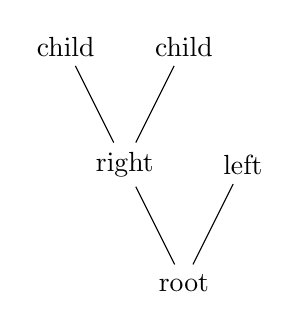
\begin{tikzpicture}
    \node {root} [grow=up]
    child {node {left}}
    child {node {right}
      child {node {child}}
      child {node {child}}
    };
\end{tikzpicture}



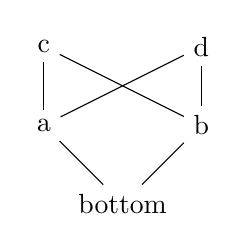
\begin{tikzpicture}
     \graph [branch right=2cm, grow up] {
        bottom [xshift=1cm] -- {
            a -- c,
            b -- d,
            b -- c,
            a -- d,
        };
    };
\end{tikzpicture}

\end{document}
